

\section{Programming with R}
\label{sec:R}
\subsection{Why R?}

In this section, we focus on introduction to data analysis and visualizations with R. After introducing the versatility of Python in the previous section, one may wonder: do we need R, and if so, why? R is one of the most popular open-source programming languages used for data analysis, visualizations and statistics. %Due to its open-source nature, the community using and contributing to R is vast.
It is widely used throughout academia in the field of statistics, which allows for new statistical methods to be made available to users quickly. Various specialized packages for data wrangling, data visualization, statistical inference, and machine learning exist, which make it a great choice for statistical analysis and experimentation. Given a data set, it is very easy to get started with R and be exploring and analyzing data in matter of minutes. Moreover, it is very well-suited for development of new algorithms and statistical methodology, as one does not need to deal with the overhead existing from complex data structures and initial set up. The goal of this chapter is to introduce the readers to data analysis and visualizations with R.

\subsection{Data Loading and Structures}
The dataset that we will be exploring is a simulated dataset of electrographic seizure and spike counts acquired from an implanted intracranial recording device. The data files are available in the GitHub repository of the book. In order to replicate the experiments below please download the data from the \verb|r_data| folder in the book's GitHub repository.

\subsubsection{Data Structures in R}
Before loading the data, we review the most common data structures used in R along with some of their benefits. As most programming languages that deal with numerical operations, R provides the users with \textbf{vector} and \textbf{matrix} structures. Atomic vectors in R can be one of four types - integer, double, Boolean/logical and character. Each atomic vector can contain only a homogeneous type of data, i.e. at most one of the four types. In contrasts, lists are similar to atomic vectors, but they can contain more than one data type. Additionally, nesting lists within lists is also acceptable in R. Atomic vectors can be extended to 2-dimensional matrices. The atomic vectors constituting the matrices are all of the same length. The matrix inherits the data structure properties of atomic vectors. The homogeneous structure of the atomic vectors and matrices allows for a trade off between computational efficiency and flexibility of storing data. To allow users the flexibility to store data from different formats, R uses \textbf{dataframes}. A dataframe is a list of vectors with the same length. Since it is a list, it allows for mixed types of data. In fact, one can store lists within a column. Additionally, dataframes can contain factors, data types used for storing categorical data in R. More recently, a newer version of dataframes, called tibbles, was introduced to R. Some of the benefits that tibbles provide are ability to use the \verb|tidyverse| \cite{tidyverse} package in R, display the data types and not loading or performing data computations until explicitly tasked to do so. This can be especially useful when manipulating large datasets. For more extensive treatment of the different data structures within R, we refer the readers to \cite{tibble} and \cite{wickham2019advanced}.

\subsubsection{Loading Datasets into R}
In many applications the data is not only stored in different file types (or databases) but some times it is divided into multiple files. The chapter covers loading such data from three distinct data types, commonly encountered - \verb|csv|, \verb|mat| and \verb|json| files. The general structure of the directory is for each patient to have a folder with all the available data. If one is to download the data from Github and place somewhere on the local drive preserving the Github structure it will be of the form \verb|./patient_data/Patient_X|, where $X$ corresponds to the patient id. The goal is to load all the data into one dataframe, which can be used for analysis and exploration.
The patient metadata files, \verb|metadata.csv|, are stored within each of the folders. A general way to load \verb|csv| files in R is via the built in function \verb|read.csv()|. To retrieve the documentation of a specific function within the R console one can invoke \verb|?| in front of it, for example, \verb|? read.csv()| will present the documentation on how to use the reader function for files with csv extension.

To load a single csv file one can do the following:
\begin{lstlisting}
# Initialize all the required paths
data_path <- "<your_path>"
single_patient_folder <- "Patient_1"
filename <- "metadata.csv"

# Concatenate all directories (as strings)
file_path <- paste(data_path, '/', single_patient_folder ,'/', filename, sep="")

# Read in the csv file for a single patient
metadata_patient1 <- read.csv(file_path, header = TRUE, sep = ",")
\end{lstlisting}
To execute the above code, one needs to change \verb|data_path <- "<your_path>"| to the folder where all the individual patient folders reside. For example, if one is using Mac OS and all the patient data folders are downloaded in \verb|"Users/Documnets/patient_data"| then this directory can be used to set \verb|data_path|.
The function \verb|read.csv()| uses the location and the filename as an input. Additionally, one can specify the headers of the csv file to be used as column names in the resulting dataframe via \verb|header=TRUE|. The variable \verb|metadata_patient1| contains the metadata for the patient corresponding to the folder \verb|Patient_1|. The loaded file is a dataframe with 1 observation, only 1 patient's metadata was loaded, and has 6 variables. Typically, when performing analysis, one is interested in looking at multiple patients. One way to load all patients is to repeat the same code from above for all patients. This can be achieved with a \verb|for loop|, where each patient's data is loaded as a new row. To accomplish this, one can create a list with all the patients folder names and execute the above code within the \verb|for loop| to load all patients. Given the folder structure, the patient list of directories can be initialized by:
\begin{lstlisting}
# Initialize a list with all patient folders
patients_list <- c()
patient_size <- 20
for (i in 1:patient_size){
  patients_list[i] <- paste('Patient_', i, sep="")

}
\end{lstlisting}
Note that lists / vectors in R can be subset by using \verb|[]| following the vector that we want to subset.
To load the metadata file from each folder into a dataframe, one can use the following code:
\begin{lstlisting}
# Initiliaze the vector where the patient's metdata will be stored
df_metadata <- data.frame()

for (i in 1:length(patients_list)){
  # Get the filepath for each patient
  file_path <- paste(data_path, patients_list[i], '/', filename, sep="")

  # Load the patient's metadata
  metadata_current_patient <- read.csv(file_path, header = TRUE, sep = ",")

  # Store the patient's metadata into a new dataframe to avoid overwriting
  df_metadata <- rbind(df_metadata, metadata_current_patient)
}
\end{lstlisting}
In the code above, the folders containing patient metadata are initialized so that 1. each one of them can be opened; 2. the data can be read in for the individual patient; and 3. stored into a final dataframe that contains the information on all $20$ patients. Note that when using \verb|for loop| in R, one must specify the condition for start and termination of the loop in parenthesis followed by the code that needs to be executed on each iteration inside \{\}.
While this illustrates well how to read in multiple csv files into one dataframe, it has some drawbacks. One, it is necessary to explicitly specify how many patients there are total via \verb|patients_size <- 20|. In certain instances, this may lead to scalability issues if one is dealing with tens of thousands of patients or even with thousands of patients. Additionally, there are built in R functions, which take advantage of lower level language, that can lead to speed improvements when compared to a \verb|for loop| in R.
To address these two the following code can be used:
\begin{lstlisting}[language=R]
# Initialize the directory containing the files and provide the filenames within each folder
files <- dir(data_path, recursive = TRUE, full.names = TRUE, pattern = "metadata.csv$")

# Iteratively load all csv files
metadata_list <- lapply(files, read.csv)
\end{lstlisting}
The built-in function \verb|dir| allows one to specify the general folder where all patient data is stored, along with the name of the file that is to be loaded. In this case one does not need to know exactly how many patient folders there are, all will be loaded. To iteratively apply \verb|read.csv| to all the folders within the data directory, one can use the function (\verb|lapply|).
Examining the output of \verb|lapply| reveals that the data was loaded as a list where the elementes are a single dataframe per loaded file. Combining the list of dataframes into a single dataframe can be achieved as follows:
\begin{lstlisting}[language=R]
# Convert the metadata to a dataframe
metadata <- data.frame(matrix(unlist(metadata_list), nrow=length(metadata_list), byrow=TRUE), stringsAsFactors=FALSE)

# Assign the appropriate column names
names(metadata) <- names(unlist(metadata_list[1]))
\end{lstlisting}

Another important file format is JSON. A lot of machine learning and software applications (especially in Python) rely on JSON files for storing data. Much like before, each patient's data is stored in a separate JSON file and interest lies in loading all files into a single dataframe. These files represent time series data on patient's spikes and seizure information. To load the JSON files and convert to a dataframe, a user defined function is created. The function is then used within \verb|lapplay| to iteratively load the data for all patients.
\begin{lstlisting}[language=R]
# Read in the json files
# Create a function for reading and processing .json files
read_json_files <- function(file_list){

  # Load json data
  rdata <- read_json(file_list, simplifyVector = TRUE)

  # Convert the large json character into a dataframe
  seizure_data <- fromJSON(rdata)

  return(seizure_data)

}

# Read in all json files
files <- dir("/Users/ev105g/Documents/temp/epilepsy_book/R_chapter/data", recursive = TRUE, full.names = TRUE, pattern = "sdata.json$")
data <- lapply(files, read_json_files)

# Convert the list of dataframes to a dataframe
seizure_data <- bind_rows(data)
\end{lstlisting}


Up to this point, only built in R functions have been used, which come with the base R distribution. However, the above code illustrates how one can 1. use functions from packages that do not come with the base R distribution and are installed on-demand; and 2. define custom functions in R, which can be used throughout the script or can be generalized and loaded for use in multiple projects. In particular, in the above code within \verb|read_json_files|, two functions are called without being explicitly defined - \verb|read_json| and \verb|fromJson|. If one is to run the code above as is, there is a good chance that the first time around, R will throw out the following error \textcolor{red}{Error in read\_json(file\_list, simplifyVector = TRUE) : could not find function "read\_json"}. This means that the currently loaded R with its distribution does not have the function present in any of its packages. A way to check what package specifically a function is part of is to use \verb|??lapply|. This function is part of the \verb|base| package in R and, hence no additional steps were required in order to call the function. However, \verb|??read_json| and \verb|??fromJSON| indicate that these particular functions are part of the \verb|jsonlite| \cite{jsonlite} package, which does not come with the base R distribution. To use the functions, the package must be installed via \verb|install.packages("jsonlite")|. The command will install the package from a remote repository onto the local drive. If one is to attempt to define \verb|read_json_files| again following the installation of the package, the same error will appear. This is because even though the package has been installed, it has not been loaded into the current R session. To do so, one must first call \verb|library(jsonlite)|. Note that the library needs to be installed only once and can then be loaded into different R sessions every time using \verb|library()|. Generally, it is helpful to have all libraries needed to execute a particular script, loaded at the beginning of the script. This highlights the true power of R - the ability to use various packages created by the ever growing R community.

The function \verb|read_json_file| is user defined and it takes one input variable \verb|file_list|. A function in R is always defined by \verb|function| followed by any arguments that the function takes contained inside \verb|()|. The instructions of the function are always enclosed inside \verb|{}|. It is a good practice, even though not required in R, to specify what is the output of the function via \verb|return()|.
Note that in the last two lines of the code above, yet, a new way to load in multiple files from multiple folders is defined. In particular, once all data is loaded into a list of dataframes, \verb|bind_rows()| from \verb|dplyr| \cite{dplyr} combines all dataframes into one. A limitation of this function is the assumption that all values within the same column in the dataframes are of the same type. For example, if one of the files, loaded as a dataframe via \verb|lapply| has, say column \verb|gender| as a string, but the second dataframe has the same column loaded as a factor, \verb|bind_rows()| will return an error. The readers can test this by applying \verb|bind_rows(metadata_list)| and exploring the results.

The final files that will be loaded are .mat files, which are usually generated from MatLab, frequently used for signal preprocessing. Each patient has the timestamps corresponding to their times of seizures and spikes recorded in the \verb|timedata.mat| files within each folder.
\begin{lstlisting}[language=R]
# Install and load the required packages
install.packages("lubridate")
install.packages("R.Matlab")
library(R.matlab)
library(lubridate)

# Read in .mat timedata file and convert to time data
files <- dir(data_path, recursive = TRUE, full.names = TRUE, pattern = "timedata.mat$")
timedata <- lapply(files, readMat)

# Check the datatype - list of strings
typeof(timedata)

# Unlist timedata to extract the characters
timedata <- unlist(timedata)

# Convert the strings to time stamps (hourly markers) using lubridate
timedata <- ymd_hms(timedata, tz="UTC")
\end{lstlisting}
To load in the MatLab files we use the \verb|readMat| function from the \verb|R.matlab| \cite{R.matlab} library. The files for each patient are iteratively loaded once again. The timestamps are stored as strings. In order to facilitate analysis and plotting, it can be useful to convert the timestamp strings to a file format that is more time series friendly. One such format is POSIXct. To conversion is performed via \verb|dmy_hms| function from the \verb|lubridate| \cite{lubridate} package. Details about the function can be found in the package documentation.

\subsection{Data Wrangling}
In this sub-section the focus is on the first steps that typical analysis takes - exploring, cleaning and joining the loaded datasets. This enables one to obtain better understanding of the data in preparation for deep dive analysis and/or modeling.

The scenario we consider here is a simplification of what a real project looks like. Typically, when performing analysis, one needs to obtain data from multiple files / databases that may or may not be in the same format. They are usually related in some way, but each also provides unique information not available in the others. The values that the data sources share in common are referred to as keys. Typically, there are two types of keys - primary and foreign keys. Primary keys refer to the column in the data that uniquely identifies a row in its own data set. A foreign key refers to the column that identifies unique values of the current data into another table/dataframe. To make these concepts more concrete, beginning the exploration of the loaded data sets is necessary.
\newline
\newline
\textbf{Initial Data Structure Exploration}
\newline
\newline
A quick way to take a look at a dataframe in R is via \textit{str()}, which retrieves some of the characteristics of the dataframe, such as number of columns, number of rows, the type of each vector and all the columns. In particular, examining the outputs of \verb|str(metadata)| and \verb|str(df_metadata)| reveals that they have loaded the same data. The exact output from \verb|str(metadata)| is:
\begin{lstlisting}[language=R]
str(metadata)
'data.frame':	20 obs. of  6 variables:
 $ ID          : chr  "Patient_1" "Patient_10" "Patient_11" "Patient_12" ...
 $ Age         : chr  "30.5" "20.9" "27.7" "26.3" ...
 $ Gender      : chr  "M" "M" "FALSE" "FALSE" ...
 $ Seizure_Foci: chr  "left frontal" "supplementary motor cortex" "right hippocampus" "left parietal" ...
 $ NA.         : chr  "2017-07-03" "2018-09-27" "2018-01-03" "2018-02-26" ...
 $ NA..1       : chr  NA NA NA NA ...
\end{lstlisting}
A subtle difference in the two dataframes is the data types of the columns. In particular, all of the columns of \verb|metadata| are strings, while \verb|df_metadata| was loaded with \verb|Age| as an integer and a column named \verb|NA..1| as a logical. Since we will be using only one of the dataframes, we can delete the other one from memory using \verb|rm(df_metadata)|. The dataframe has 20 observations and 6 variables. The column \verb|ID| is the primary key for the dataframe as it is able to uniquely define the rows.

The output to \verb|str(seizure_data)| is:
\begin{lstlisting}[language=R]
str(seizure_data)
'data.frame':	40000 obs. of  5 variables:
 $ iea_lead1     : int  0 0 0 0 0 0 0 0 0 0 ...
 $ iea_lead2     : int  0 0 0 0 1 2 0 3 0 2 ...
 $ LE            : int  0 0 0 0 0 0 1 0 0 0 ...
 $ patient_id    : int  1 1 1 1 1 1 1 1 1 1 ...
\end{lstlisting}
The dataframe has 40,000 observations of 4 variables. The variables are all integers. The column \verb|le| corresponds to the number of seizures within the one hour time window defined in \verb|timedata|. Similarly, \verb|iea_lead1| and \verb|iea_lead2| correspond to the number of spikes for each one hour window, recorded by each of the two leads. The unique key in this case consists of multiple columns. The column \verb|patient_id| no longer uniquely identifies each row and the primary key must be defined by multiple columns. To identify the rows uniquely, the dataframe needs to be combined with \verb|timedata|. The primary keys for the combined dataset are \verb|patient_id| and the timestamps.
\newline
\newline
\textbf{Joining Data Frames}
\newline
\newline
The simplest way of adding a column to a dataframe in R consists of \verb|seizure_data$hourly_markers <- timedata|. Two items are of note here, 1. adding new columns or updating existing columns to/in a dataframe can be achieved by using \verb|$| symbol following the dataframe name and 2. assigning the timestamps in such a way may be dangerous, because it assumes that the order of the values in the \verb|seizure_data| dataframe is aligned with the order of values in the \verb|timedata| variable. In this instance, this is not an issue due to the nature of the data, but in what follows more robust methods for handling data joining are presented.
Often times, when performing analyses or building supervised / unsupervised learning models, it is more convenient to combine all the data into a single dataframe. To combine two dataframes in R, taking advantage of the relational nature of the data, one can use \verb|merge|. The readers are encouraged to explore the documentation \verb|?merge| for additional details beyond what is outlined here. The primary keys from each dataframe, \verb|patient_id| and \verb|ID| are stored as different structures, a character and an integer. Before joining the two dataframes it is necessary to convert both primary keys to the same data structure in order to avoid faulty joins. The \verb|ID| column in \verb|metadata| has the patient id, preceded by the string 'Patient\_'. In this case, for pedagogical purposes, the \verb|patient_id| column will be converted to match \verb|ID| rather than vice-versa. In the following section we discuss strategies for obtaining a sub-string of a string which can also be applied to convert \verb|ID| into an integer format containing the patient id only.
\begin{lstlisting}[language=R]
seizure_data$patient_id <- paste0("Patient_", seizure_data$patient_id)
\end{lstlisting}
To join the two dataframes:
\begin{lstlisting}[language=R]
# Join the metadata into the dataframe
seizure_data <- merge(seizure_data, metadata, by.x = 'patient_id', by.y = 'ID', all.x = TRUE, all.y = FALSE)
\end{lstlisting}
The function expects as inputs the two dataframes that are to be joined, the keys from each data frame that we join on and how to join the two dataframes. In this case the key used for joining the two dataframes is the single column \verb|patient_id| contained in each of the dataframes. Note that in this case the primary keys from the dataframes have different names and hence one must explicitly state them via \verb|by.x| and \verb|by.y|. The use of \verb|by='patient_id'| is valid, provided that the column names are identically named \verb|patient_id| in both dataframes. Moreover, while in this example only one column was needed to join the dataframes, in other cases, when multiple keys need to be joined, they can be specified by passing a vector via \verb|by = c(join_column1, join_column2, ... )|.
Finally, a left join, which joins so that if a key value in the \verb|seizure_data| does not have a matching record in the \verb|metadata| dataframe the row is still returned, with all seizure columns with their original values and \verb|NA| for the values in the metadata column(s). To accomplish this with \verb|merge|, one specifies \verb|all.x=TRUE| and \verb|all.y = FALSE|. When using a left join the resulting dataframe has the same number of rows as the first (left) dataframe passed to \verb|merge|. This can be verified by running \verb|str(seizure_data)|. The merged dataframe has 40,000 rows and 10 columns. This new dataframe contains all the data that is available. Another useful way of joining datasets is to perform an inner join. In an inner join, only the rows that have matches in both dataframes are returned. Using \verb|merge| in R, an inner join can be performed by setting \verb|all.x=TRUE| and \verb|all.y = TRUE|.
\newline
\newline
\textbf{Data Cleaning}
\newline
\newline
After joining all datasets into a single dataframe, tools for cleaning and formatting data enable one to perform exploratory data analysis and modeling. The \verb|str| command quickly reveals a few issues with the data. As previously discussed \verb|Age| was read in as a character. In this case age is entered as a decimal and hence, converting it to a numeric value is advisable:
\begin{lstlisting}[language=R]
# Convert age and patient_id columns from strings to floats
seizure_data$Age <- as.numeric(seizure_data$Age)
\end{lstlisting}
If the age was entered as an integer one can convert using \verb|as.integet()|

Further, some of the column names are capitalized, while others are lower case letters. For consistency, one can change all column names to lower case by:
\begin{lstlisting}[language=R]
# Change the column names to lowercase letters
names(seizure_data) <- tolower(names(seizure_data))
\end{lstlisting}

Exploring \verb|gender|, one may find that it contains two values - \verb|FALSE| and \verb|M|. It is safe to assume that the former is a result of reading in the data incorrectly and the entry should be \verb|F| representing female, rather than the boolean value \verb|FALSE| read in as a string. Before addressing this issue, it may be useful to check the unique values in the gender column. One way to achieve this is via \verb|unique(seizure_data$gender)|, which confirms the existence of only two unique values in the column. There are several ways to convert \verb|FALSE| to \verb|F| to match more standard representations. As an example, one can use \verb|gsub("FALSE", "F", seizure_data$gender)|. The function will find all occurrences of the first string, replace it with the second and insert it into the \verb|gender| column in the dataframe \verb|seizure_data|. The same outcome can be accomplished the same way using \verb|stri_replace_all_fixed(seizure_data$gender, "FALSE", "F")| from the \verb|stringi| \cite{stringi} package. Since both functions accomplish the same outcome, a natural question is which one should be used. One way to answer this question is to compare the execution time of each function applied to the dataframe:
\begin{lstlisting}[language=R]
install.packages('microbenchmark')
install.packages('stringi')
library(microbenchmark)
library(stringi)
microbenchmark(gsub("FALSE", "F", seizure_data$gender), stri_replace_all_fixed(seizure_data$gender, "FALSE", "F"))
\end{lstlisting}
The produced output is:
\begin{table}[h]
  \centering
  \label{tab:execution_time}
  \begin{tabular}{lrrrrrrr}
    \hline
    expr & min & lq & mean & median & uq & max & neval \\
    \hline
    gsub & 15.02 & 15.64 & 16.19 & 16.12 & 16.41 & 21.44 & 100 \\
    stringi & 5.29 & 5.60 & 5.96 & 5.74 & 5.92 & 19.15 & 100 \\
    \hline
  \end{tabular}
  \caption{Execution Time in Milliseconds over 100 trials}
  \label{tbl:substr}
\end{table}
From table \ref{tbl:substr}, \verb|stri_replace_all_fixed| is about 3x faster than gsub. Generally, this advantage can further increase for larger datasets. An important point here is that given the amount of packages available such comparisons can be very useful to make sure that the best function for the dataset at hand is used.

Converting \verb|"FALSE"| to \verb|"F"| within \verb|gender| and updating the column within \verb|seizure_data| is achieved via:
\begin{lstlisting}[language=R]
seizure_data$gender <- stri_replace_all_fixed(seizure_data$gender, "FALSE", "F")
\end{lstlisting}

%%% We are here
There are two columns in the dataset that have column names \verb|na.| and \verb|na..1|. The values in the former are dates, which represent the first visit date for each patient. To rename the column, one can use:
\begin{lstlisting}[language=R]
# Change column names
col_names <- colnames(seizure_data)
colnames(seizure_data)[col_names == "na."] <- 'first_visit_date'
\end{lstlisting}
The original column name \verb|na.| has been replaced with \verb|first_visit_date| which is much more informative relative to the values it represents.
Before renaming the column name \verb|na..1| it is worth exploring its content, given that the first few values are \verb|NA|. Executing \verb|unique(seizure_data$na..1| returns only \verb|NA|. The column contains no useful values that can be used for analysis and is most likely an artifact of data loading or issues with file formats. In such instances it is best to drop the column to save memory and to clean up the dataset. One way of dropping a column in R is to use the subset operator:
\begin{lstlisting}[language=R]
# Drop the column using the subset operator
seizure_data <- seizure_data[, -which(names(seizure_data) == "na..1")]
\end{lstlisting}
The inner most argument, checks which column name(s) are \verb|na..1|. \verb|which()| returns the index of the column satisfying that condition. To subset the data, all rows and all the complement (implemented via the "-" sign here) indices of the column name being \verb|na..1| are taken.

In this instance, it was easy to spot \verb|NA| in the data, because the first few rows were populated with missing values. This is not always the case. Some times the \verb|NA| can be a small percentage of the data and may be spread out throughout the rows. Therefore, a more programmatic way for checking all the rows for missing values is needed. To that end a user defined function is introduced below. It takes two inputs, a dataframe and a threshold value. The output is all columns along with proportion of missing values above the user input threshold.
\begin{lstlisting}[language=R]
# Define a function for displaying all columns that have NA
display_na <- function(df, threshold){
  # Params:
  # df: data.frame - data frame for which the NA percentage is to be calculated
  # threshold: double - value between 0 and 1 indicating that columns with NA
  #                     proportion higher than threshold should be returned

  # Return:
  # named vector with all columns that have more than threshold proportion of values with NA

  na_percent_per_column <- round(colMeans(is.na(df)),3)
  return(na_percent_per_column[na_percent_per_column > threshold])
}

# Apply the custom defined NA function
display_na(seizure_data, 0.01)
le   iea_lead1  iea_lead2
0.1     0.1       0.1
\end{lstlisting}
In the user defined function we have added a doc string describing the input parameters and the returned values from the function. Adding doc string is a very common and useful practice to enable users of the function to know the inputs/outputs and their data structures. The first line in the executable code determines what values in the dataframe are \verb|NA|; \verb|colMeans()| is used to calculate the average of a binary dataframe which returns percent of \verb|NA| for each column. The second line returns only the columns and their \verb|NA| percentage that exceed the user provided threshold. Applying the function to the seizure dataset, returns three columns which exceed the user defined threshold of 0.01, namely seizures and each of the lead locations. Each of the columns has the same missing percentage - 10\%.
There are different ways to treat missing values, and their details are beyond the scope of this chapter, however, the methods used to apply them in R are explore below.
The simplest way to treat \verb|NA| is to drop the entire row if any of the columns contain it.
\begin{lstlisting}[language=R]
# If NA is present in any row of the entire dataframe drop that row
any_na_drop = na.omit(seizure_data)
\end{lstlisting}
Checking the dimension of \verb|any_na_drop| indicates that the new dataframe has 36,000 rows. This indicates that about ~10\% of the data has been discarded as expected. In this case the dataframe is relatively large and losing that many observations may not be a big issue when trying to get inference or model the data. However, in instances where the data has small sample size, losing 10\% of the data can be critical. Another observation that can be made is that since any row that contains \verb|NA| was dropped, and exactly 10\% of the data was lost, implies that the rows across the three variables that contain missing values coincide. Note that this must not always be the case.
A second way of removing missing values is by specifying the columns which all must contain \verb|NA| to be removed.
\begin{lstlisting}[language=R]
partial_na_drop = seizure_data[complete.cases(seizure_data[, 2:4]),]
\end{lstlisting}
The code above uses \verb|complete.cases()| to remove the missing values. In this case rows with missing values are dropped if columns 2, 3 and 4, which correspond to \verb|le|, \verb|iea_lead1| and \verb|iea_lead2|, are missing. The dimension of \verb|partial_na_drop| is the same as \verb|any_na_drop| further confirming that the three columns related to seizures and lead locations are either all missing or are all available.

The final method for handling missing values that is considered here is imputation. While there are many ways to perform imputation \cite{buuren2018flexible}, here median value imputation is presented. In particular, the median for each column is calculated from the non-missing values, and all \verb|NA| are subsequently replaced with that value. To achieve this two more functions are defined below. The first one takes a vector of values and replaces all missing values in the vector with the median. The second function takes in a dataframe and a general imputation function as an input and returns the dataframe with the missing values imputed with the input function.
\begin{lstlisting}[language=R]
# Create a function for filling NAs with median
median_noNA <- function(df){
  # Return the median value of x removing NA
  return(replace(df, is.na(df), median(df, na.rm = TRUE)))
}

# Execute the function on each row in the dataframe
replace_na <- function(df, impute_function){

  # Get only the numeric columns
  is_numeric <- sapply(df, is.numeric)

  # Impute NA inplace with the median
  clean_df <- replace(df, is_numeric, lapply(df[is_numeric], impute_function))
  return(clean_df)
}
\end{lstlisting}
Note the use of the function \verb|replace|, which takes a vector, a list of indices on which to operate and values to use to replace the dataframe.
The missing values can be imputed via:
\begin{lstlisting}[language=R]
# Impute missing values in place
seizure_data_median_impute = replace_na(seizure_data, median_noNA)
\end{lstlisting}
The general modular structure of both functions allows for easily adding other functions that can be used for imputing the missing values. For example, if one would like to impute the missing values with the mean instead of median, it is as simple as defining:
\begin{lstlisting}[language=R]
mean_noNA <- function(df){
  # Return the mean value of x removing NA
  return(replace(df, is.na(df), mean(df, na.rm = TRUE)))
}
\end{lstlisting}
and then reusing \verb|replace_na(seizure_data, mean_noNA)|. Code reusability and designing software so that it is not only easy to understand and maintain, but also easy to extend are very important aspects of software engineering and we encourage the readers to always keep that in mind when designing their projects and code repositories and scripts. To check whether we have treated the missing values problem one can run \verb|display_na(seizure_data_median_impute, 0.01)| which should return no columns if the imputation was successful.

Even though custom functions were defined here to impute missing values, there are a lot of libraries developed by the R community that can handle missing values. For example, imputing the missing values can be achieved using \verb|mutate_at| from \verb|dplyr|:
\begin{lstlisting}[language=R]
seizure_data <- seizure_data %>%
  mutate_at(vars(c(le, iea_lead1, iea_lead2)), ~ifelse(is.na(.), median(., na.rm = TRUE), .))
\end{lstlisting}
The columns to be imputed have been explicitly stated. This may not scale well if there are hundreds of columns that need to be imputed. In these instances extracting the columns from the dataframe in a programmatic way is advisable. The readers are encouraged to explore \verb|?mutate_at| to learn more about the function.

As each of the individual lead columns represents the number of spikes within that lead, it may be useful for analysis purposes to combine the two variables into one, add it to the dataframe and drop the individual variables.
\begin{lstlisting}[language=R]
# Add the two leads and use the aggregated variable. Drop the individual ones
seizure_data$iea_lead_agg = seizure_data$iea_lead1 + seizure_data$iea_lead2
seizure_data <- subset(seizure_data, select = -c(iea_lead1,iea_lead2) )
\end{lstlisting}
Each of the columns is a numeric value and hence addition can be performed as adding any vectors or scalar values. Once the combined number of seizures is stored into the dataframe, dropping the individual ones can be achieved by subsetting the complement of these two columns. While, previously a subset operator was used, now the subset function is used. The subset operator will be valid here as well.

\subsection{Exploratory Data Analysis}
Typically, once the data cleaning and preparation is complete, in depth data exploration can begin to uncover the underlying data structure and relationships. Frequently, the exploratory data analysis can reveal further data cleaning and transformation that is necessary, as more of the data structure is revealed. Further, the two can be intertwined as we have already explored some of the data in the previous sub-section while cleaning and preparing the data.

A good starting point is exploring the distribution of the main variables of interest - seizure counts (\verb|le|) and seizure spikes (\verb|iea_lead_agg|. To explore the data one can build a histogram of each variable in R via:
\begin{lstlisting}[language=R]
# Plot histograms for LE (seizure counts) and IEA Leads (seizure spikes)
hist(seizure_data$le, main = "", xlab = "Seizures", ylab = "Density", freq=FALSE)
hist(seizure_data$iea_lead_agg, main = "", xlab = "Seizure Spikes", ylab = "Density", freq=FALSE)
\end{lstlisting}
The resulting histograms Figure \ref{fig:seizures} indicate that the majority of the seizure counts are 0. Moreover, for each hour each patient has at most one seizure. Similarly, the majority of seizure spikes for each hour are 0. However, there are more seizure spikes per hour than seizures. It looks like the density of the seizure spikes is right-skewed and is tapering off after 100 with very few seizure spikes above 200.
\begin{figure}
  \begin{minipage}[b]{0.5\linewidth}
    \centering
     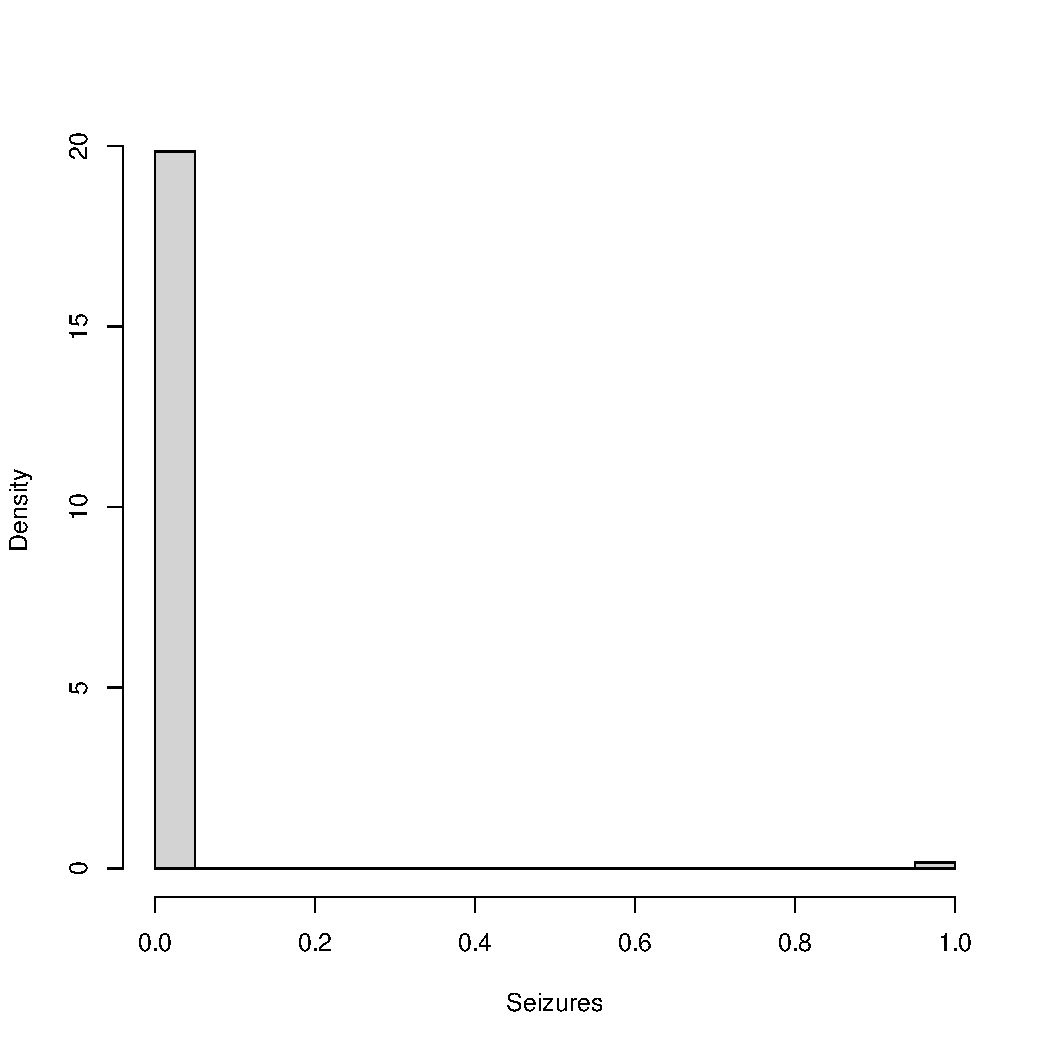
\includegraphics[width=\linewidth]{chapters/CodingBasics/figures/le_histogram.pdf}

  \end{minipage}
  \begin{minipage}[b]{0.5\linewidth}
    \centering
     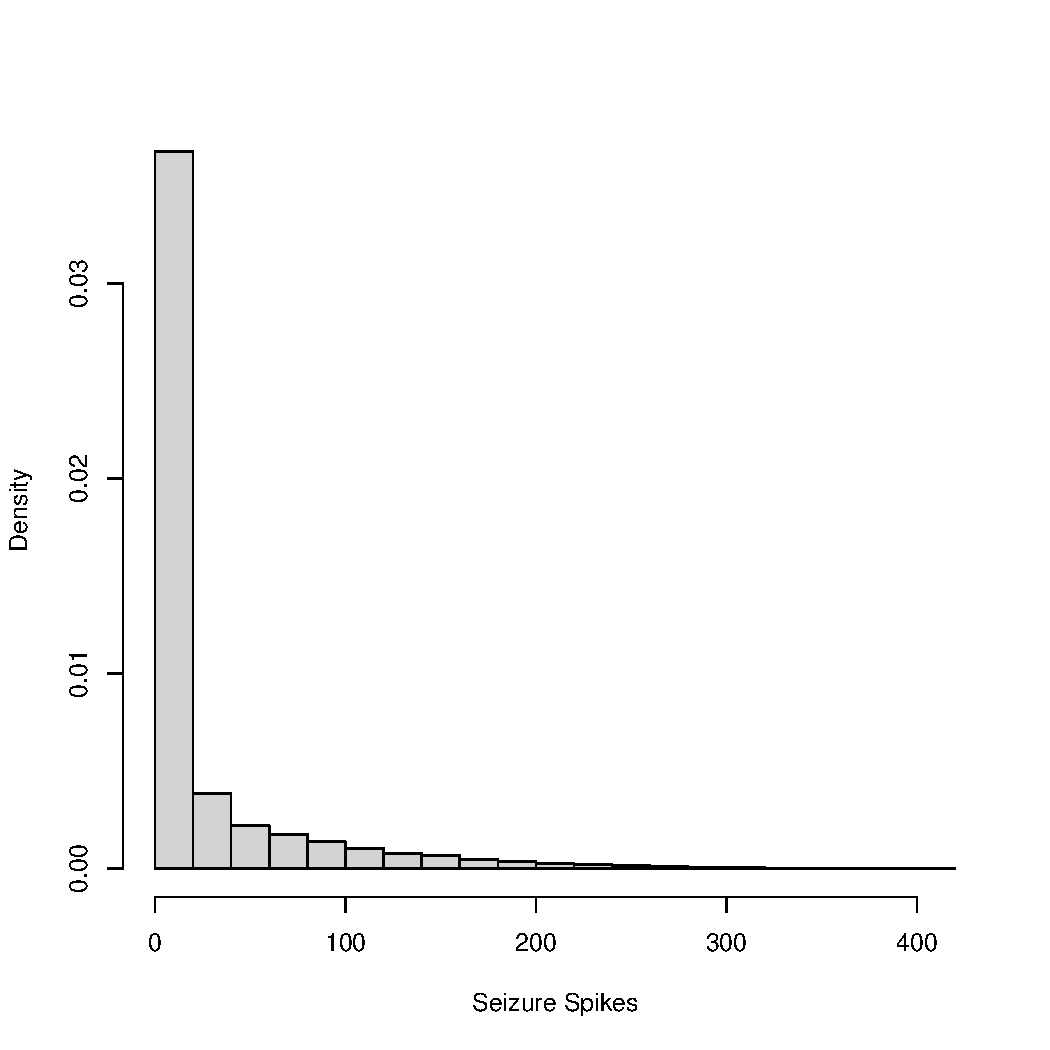
\includegraphics[width=\linewidth]{chapters/CodingBasics/figures/iea_lead_agg.pdf}
  \end{minipage}
  \label{fig:seizures}
  \caption{Histograms of seizures for every hour across all patients (left) and seizure spikes for every hour across all patients (right)}
\end{figure}
An alternative way to explore the distribution of a variable is to use \verb|summary(seizure_data$iea_lead_agg)| which results in the following output:
\begin{lstlisting}[language=R]
Min. 1st Qu.  Median    Mean 3rd Qu.    Max.
0.00    1.00    6.00   26.05   22.00  406.00
\end{lstlisting}
The results confirm some of the earlier observations, of right skewness, given the discrepancy between the median and the mean values. The maximum number of seizure spikes in one hour period is $406$. However, $75\%$ of the data has less than $22$ seizure spikes in one hour interval.
To further explore the distribution of the seizures and seizure spikes, one may want to aggregate the data on a daily basis rather than hourly. This can be accomplished by summing across the timestamps within each hour.
\begin{lstlisting}[language=R]
# Extract the dates from the time stamps
seizure_data$seizure_date <- as.Date(seizure_data$hourly_markers)

# Aggregate the seizures and spikes on daily level into a new dataframe
daily_seizures_spikes <- seizure_data %>%
  group_by(patient_id, seizure_date) %>%
  summarise(total_le = sum(le), total_iea_lead_agg = sum(iea_lead_agg))

# Plot the histograms
hist(daily_seizures_spikes$total_le, main = "", xlab = "Seizures", ylab = "Density", freq=FALSE)
hist(daily_seizures_spikes$total_iea_lead_agg, main = "", xlab = "Seizure Spikes", ylab = "Density", freq=FALSE)
\end{lstlisting}
In the first line \verb|as.Date()| extracts the date from the timestamp and assigns it to \verb|seizure_date|. The second block of code uses the \verb|dplyr| convention to group the dataframe by patient id and the date in which the seizure took place and then aggregates, by summing across all seizures and all seizure spikes, for each group. The result is a new dataframe, \verb|daily_seizures|, which has 1,686 observations and 4 columns, containing the patient id, the seizure date (extracted from the timestamp), the total seizures (\verb|total_le|) per day and the total spikes per day (\verb|total_iea_lead_agg|). The histogram of the daily seizures and spikes is presented in figure \ref{fig:daily_seizures}. The distribution of the seizure spikes seems similar to what was seen before, except that now the values per day are much larger (figure \ref{fig:daily_seizures} right). The left figure shows that even though overall most patients did not experience any seizures on a given day. The maximum seizures that a patient has had in a day is $8$.
\begin{figure}
  \begin{minipage}[b]{0.5\linewidth}
    \centering
     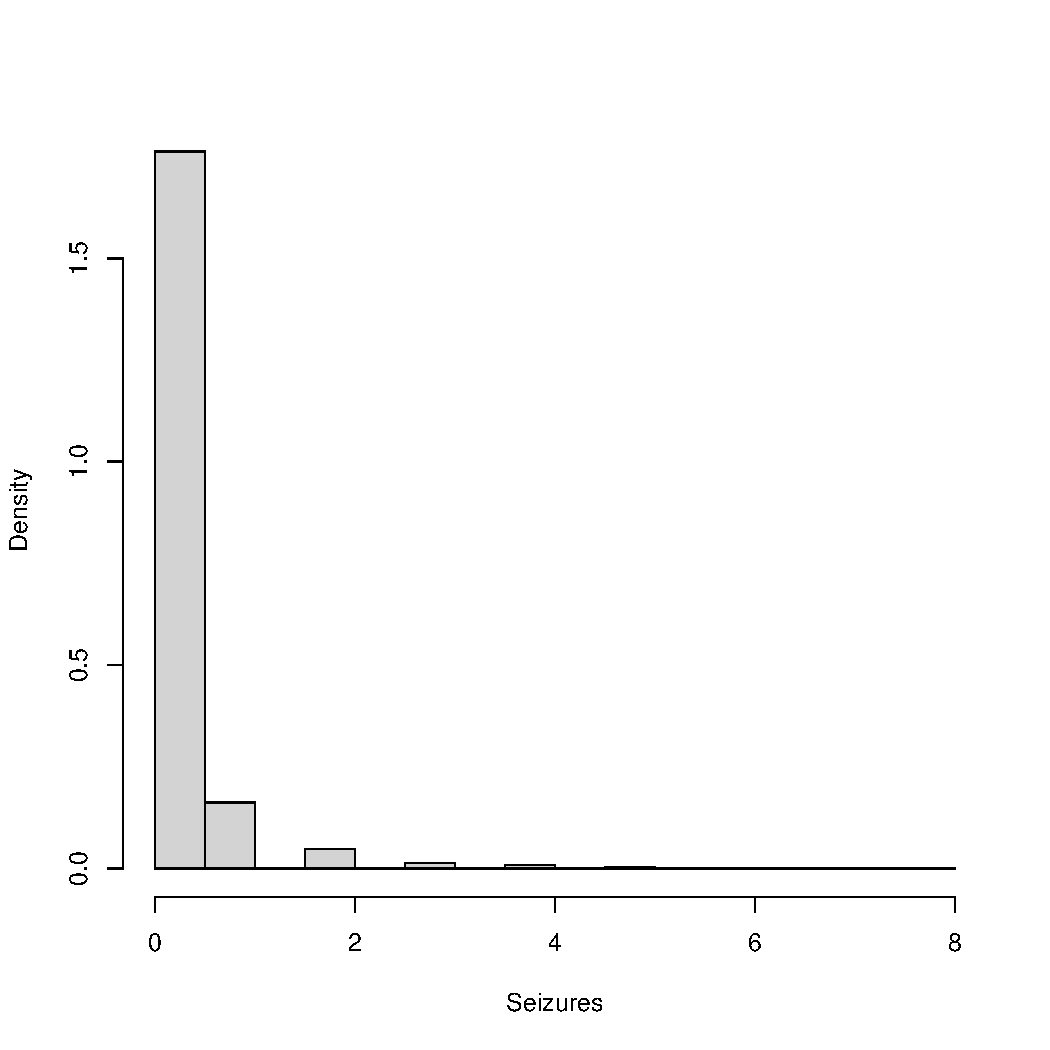
\includegraphics[width=\linewidth]{chapters/CodingBasics/figures/daily_le_histogram.pdf}

  \end{minipage}
  \begin{minipage}[b]{0.5\linewidth}
    \centering
     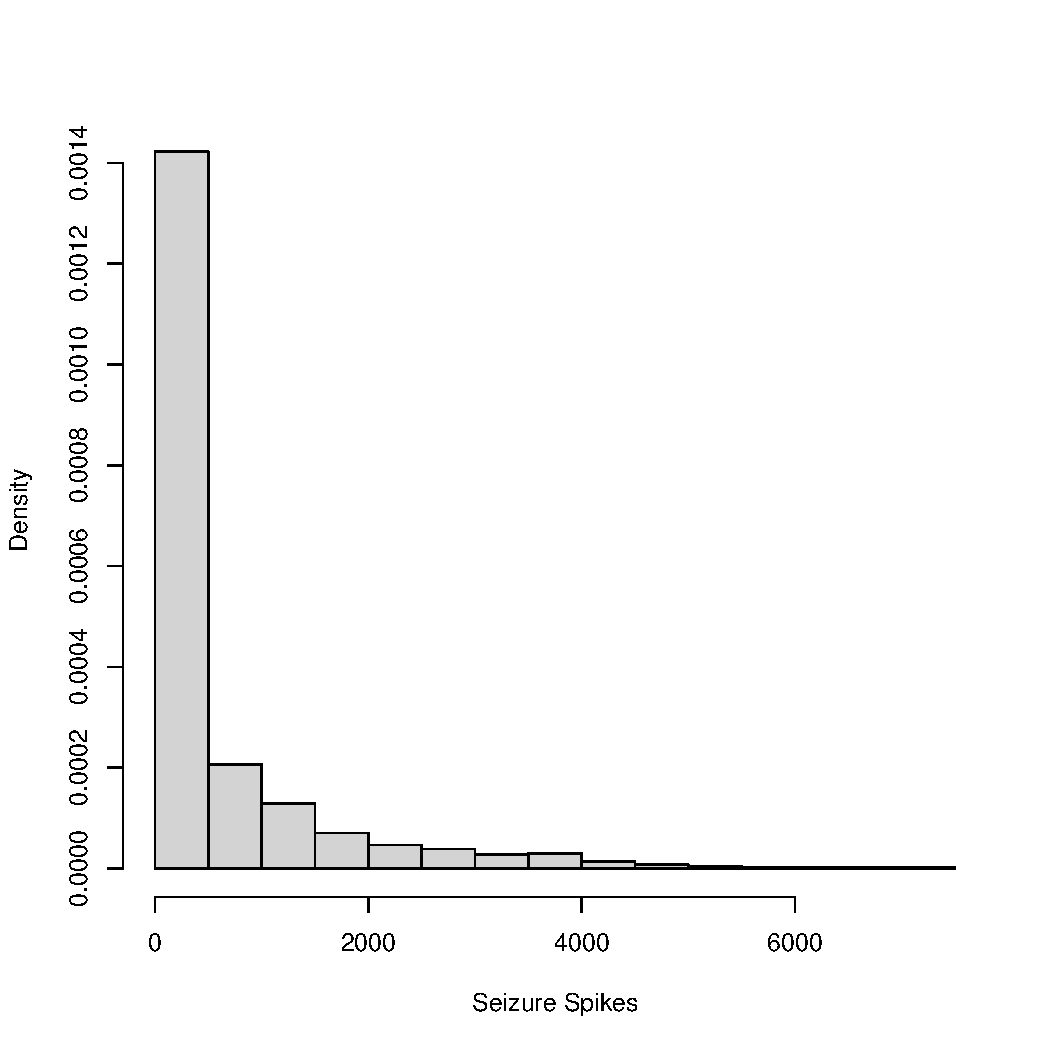
\includegraphics[width=\linewidth]{chapters/CodingBasics/figures/daily_iea_lead_agg.pdf}
  \end{minipage}
  \label{fig:daily_seizures}
  \caption{Histograms of seizures for every day across all patients (left) and seizure spikes for every day across all patients (right)}
\end{figure}

%We are here
Another variable of interest is \verb|seizure_foci|. The overview of the \verb|seizure_data| dataframe earlier indicated that it is a character variable. To check its unique values, once again one can invoke \verb|unique(dataframe$seizure_foci)|. The output indicates that there are eight different values - left frontal, supplementary motor cortex, right hippocampus, left parietal, left postcentral gyrus, left hippocampus, left insula, right frontal.

To check whether each of the eight seizure foci occurs across each patient
\begin{lstlisting}[language=R]
seizure_data %>%
  group_by(patient_id) %>%
  summarise(count = n_distinct(seizure_foci))
\end{lstlisting}
The result is a \verb|tibble| outputting the number of distinct seizure foci per patient. It looks that each patient has exactly one seizure focus. {SHARON CAN YOU DISCISS IF THIS IS NORMAL??? SURPRISING? SOME COMMENTS HERE?}.
To output the patient id for each seizure focus one can use:
\begin{lstlisting}[language=R]
aggregate(patient_id ~ seizure_foci, seizure_data, function(x) paste(unique(x), collapse = ", "))
\end{lstlisting}
The \verb|aggregate()| function allows to specify how the data should be exactly subset and what function should be applied to each group. In this case, the code specifies that for each patient id, the unique seizure foci should be returned. Note the way one can define a function inside \verb|aggregate| to incorporate an existing function within the grouping. In this case \verb|unique| is used. For more information on how to use the function the readers are encouraged to search the documentation via \verb|?aggregate|. Table \ref{tab:seizure_foci} shows the results of the aggregation:
\begin{table}[ht]
\centering
\begin{tabularx}{\textwidth}{|l|X|}
\hline
Seizure Foci                   & Patient ID \\ \hline
left frontal                   & Patient\_1 \\ \hline
left hippocampus               & Patient\_2, Patient\_6, Patient\_9 \\ \hline
left insula                    & Patient\_20 \\ \hline
left parietal                  & Patient\_12 \\ \hline
left postcentral gyrus         & Patient\_19, Patient\_8 \\ \hline
right frontal                  & Patient\_5 \\ \hline
right hippocampus              & Patient\_11, Patient\_13, Patient\_14, Patient\_15, Patient\_18, Patient\_3, Patient\_4, Patient\_7 \\ \hline
supplementary motor cortex     & Patient\_10, Patient\_16, Patient\_17 \\ \hline
\end{tabularx}
\caption{Seizure focus locations and the corresponding patient IDs.}
\label{tab:seizure_foci}
\end{table}
The majority of the patients have the right hippocampus as their epileptogenic zone. {SHARON CAN YOU DISCISS IF THIS IS NORMAL??? SURPRISING? SOME COMMENTS HERE?}. The second most common seizure foci are left hippocampus and the supplementary motor cortex.

While performing analysis, often times it is useful to convert string valued variables to factors, a format frequently used in R. Moreover, most statistical models for inference or machine learning models expect the inputs to be numeric. While some libraries perform the conversion in the background and the user is allowed to pass character valued vectors to the function, it is never the case that these strings are directly input into the model training functions. There are two columns that are candidates for being converted to factor columns - \verb|gender| and \verb|seizure_foci|.
\begin{lstlisting}[language=R]
# Convert the gender and seizure foci columns to factors
factor_cols <- c('gender', 'seizure_foci')
seizure_data[factor_cols] <- lapply(seizure_data[factor_cols], factor)
\end{lstlisting}
Inspecting the dataframe confirms that the \verb|gender| and \verb|seizure_foci| columns have been converted to factors with two and eight levels, respectively.
As the seizure data frame is a time series data, it is interesting to study the seizures and spikes over time. To this end, exploration of the time component of the dataframe is presented below. To check the minimum and maximum dates for the time series, one can use \verb|min(seizure_data$hourly_markers)| and \verb|max(seizure_data$hourly_markers)|. The timestamps range from 2017-01-05 to 2019-04-14.
Since the dataframe contains data on all patients one can explore the number of observations per patient by grouping all unique time stamps for each patient:
\begin{lstlisting}[language=R]
seizure_data %>%
  group_by(patient_id) %>%
  summarise(count = n_distinct(hourly_markers))
\end{lstlisting}
The results indicate that all patients have around 2000 distinct observations. Patients with IDs 2 and 5 have 1999 distinct observations each. This is indicative of duplicates in the data. The following code serves to drop the duplicate observations:
\begin{lstlisting}[language=R]
# Drop duplicate observations
seizure_data <- seizure_data[!duplicated(seizure_data), ]
\end{lstlisting}
Often times, clinical interest lies in understanding and predicting seizures over time, which can lead to better treatment outcomes. To this end, a good first step in is visualizing and obtaining better understanding of the the time structure of the seizure and spikes data. To look at an individual patient's time series, one can subset the seizure dataframe. In particular to subset the data for Patient 6:
% We are here
\begin{lstlisting}[language=R]
seizure_data_2017_patient_6 <- seizure_data[seizure_data$patient_id == 'Patient_6', ]
\end{lstlisting}
Since the hourly series contains nearly 2000 observations, for visualization purposes, the focus is on a shorter time interval that is known to contain seizures. In particular, to extract the patient's spikes and seizures for the time period February 1, 2017 to March 20, 2017 one can use:
\begin{lstlisting}[language=R]
seizure_data_subset_2017_patient_6 <- seizure_data_2017_patient_6[(seizure_data_2017_patient_6$hourly_markers > '2017-02-01 00:00:00 UTC') & (seizure_data_2017_patient_6$hourly_markers <= '2017-03-20 00:00:00 UTC'),]
\end{lstlisting}
In this case there are two conditions to subset on. They can be chained together within parenthesis and separated by \verb|&| indicating that both conditions need to be met for the condition to be true.
Figure \ref{fig:time_seizure_spikes} displays the number of spikes for each one hour period for the dates specified above. The red dots represent the seizures within the same time frame.
\begin{figure}[H]
  \centering
   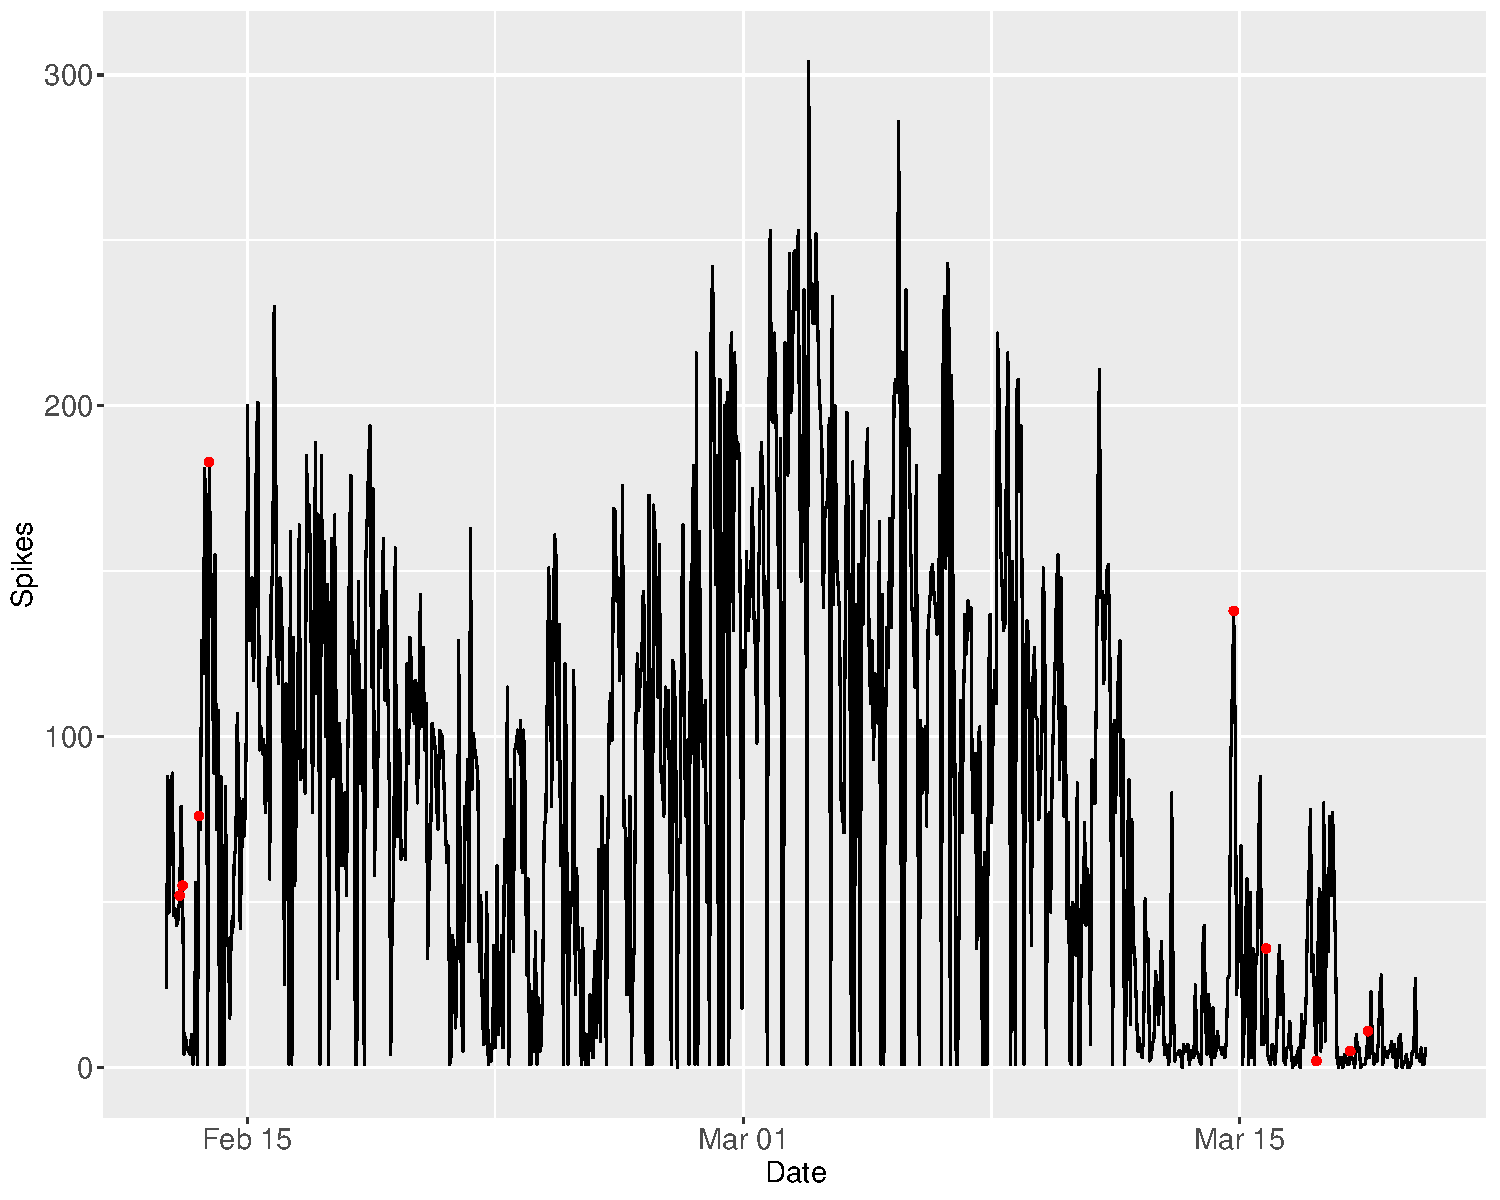
\includegraphics[width=\textwidth]{chapters/CodingBasics/figures/hourly_seizure_spikes.pdf}
  \caption{Hourly spikes (solid black lines) and seizures (red dots) for a sample patient.}
  \label{fig:time_seizure_spikes}
\end{figure}
The figure can be reproduced via:
\begin{lstlisting}[language=R]
install.packages(ggplot2)
library(ggplot2)
# Create a plot for the spikes
spikes <- ggplot() +
  geom_line(data=seizure_data_subset_2017_patient_6, aes(x=hourly_markers, y=iea_lead_agg)) +
  xlab("Date") +
  ylab("Spikes")

# Add the seizures as dots to the plot
spikes + geom_point(data=seizure_data_subset_2017_patient_6[seizure_data_subset_2017_patient_6$le > 0, ], aes(x=hourly_markers, y=iea_lead_agg), color='red')
\end{lstlisting}
To produce the figure, the \verb|ggplot2| \cite{ggplot2} library has been utilized. The readers are encouraged to browse through the documentation for it as it is one of the most widely used R libraries for creating visualizations.
The spikes exhibit large variability over time, ranging from 0 to 300 per hour, with a mean of about 82. There are signs of cycles over time. In particular, spikes increase throughout early and middle part of February followed by a decrease heading into March. Then the number of spikes increases again followed by a decrease starting around March 10. \textcolor{red}{SHARON CAN YOU COMMENT ON FIGURE 3 MORE???}. For the plotted time period, the patient has a total of nine seizures as indicated by the red dots. The seizures exhibit clustering patterns with four of the nine occurring at the beginning of the time period, Feb 1 - Feb 15, and the other five between March 15 and March 20. (\textcolor{red}{SHARON ARE THERE REFERENCES FOR THIS??? CAN YOU COMMENT MORE ON THIS???}. An additional observation here is that the majority of the seizures occur on the upper trajectory of the spikes observed in the time series. \textcolor{red}{SHARON CAN YOU PROVIDE REFERENCE FOR DR RAO STUDY AND COMMENT MORE ON THIS PHENOMENON???}
The readers are encouraged to repeat this analysis for other patients as well.
